\documentclass{beamer}
\usetheme{CWRU}

\title{Exploring Alternative Routes Using Multipath TCP}
\author{Stephen Brennan}
\institute{Case Western Reserve University}
\date{June 5, 2017}

\usepackage{appendixnumberbeamer}
\usepackage{pgfpages}
\usepackage{wrapfig}
\usepackage[export]{adjustbox}
\usepackage{graphicx}
\setbeamertemplate{note page}[plain]
\setbeameroption{show notes on second screen=right}
\setbeamertemplate{navigation symbols}{}%remove navigation symbols

\newcommand{\FigureSlide}[2]{
  \begin{frame}[plain]
    \includegraphics[max width=\textwidth,max height=\textheight]{#1}
    \note{#2}
  \end{frame}
}

\begin{document}
\frame{
  \titlepage
  \note{
    Hello everyone. I'm Stephen, and today I'll be discussing my thesis,
    entitled ``Exploring Alternative Routes Using Multipath TCP''.
  }
}

\begin{frame}{Overview}
  \tableofcontents
  \note{
    Here is how this talk is going to be structured. First, I'll be giving a bit
    of motivation for this project, along with a problem statement and our
    background information. Next, I'll discuss related work in this field, and
    show how this thesis fits into the current research. After that, I'll give
    an overview of the implementation of the components of the thesis. Next,
    I'll discuss the experiments I used to validate the mechanism, and finally
    we'll conclude with a brief summary and discussion of future work.
  }
\end{frame}

\section{Introduction}

\FigureSlide{figures/InternetSlide.pdf}{
  Okay, so let's get started! I want to start off with a brief and simplified
  look at the Internet. As we know, the Internet is made up of routers, the blue
  dots, and Autonomous Systems, the tan groups. The task of each router is to
  forward small packets of information toward their final destination. The route
  that packets take is determined by a lot of factors.

  While this project isn't directly about routing, let's discuss some of these
  factors. Routing is typically performed, in some way or another, by an
  application of Dijkstra's algorithm for finding a shortest path. While this
  might be optimal in a theoretical sense, the practical application is not, and
  for several reasons.

  For one, routing algorithms are going to work by ``hop count'',
  meaning that a shorter path should be preferred, even if the longer path might
  actually exhibit better properties. For another, the Autonomous Systems are
  frequently businesses or ISPs, and the connections they make are determined by
  business agreements. They may create policies that are less than optimal in
  order to fulfill business objectives.
}

\begin{frame}
  \frametitle{Internet Routing Inefficiencies}
  \begin{columns}
  \begin{column}{0.7\textwidth}
  \begin{itemize}
  \item The default route is not always the best, in terms of latency or
    reliability
  \item Peering agreements and policy based routing can result in suboptimal
    routing decisions \cite{detour}
  \item A route that passes through a ``detour'' may be better
  \end{itemize}
  \end{column}
  \begin{column}{0.3\textwidth}
    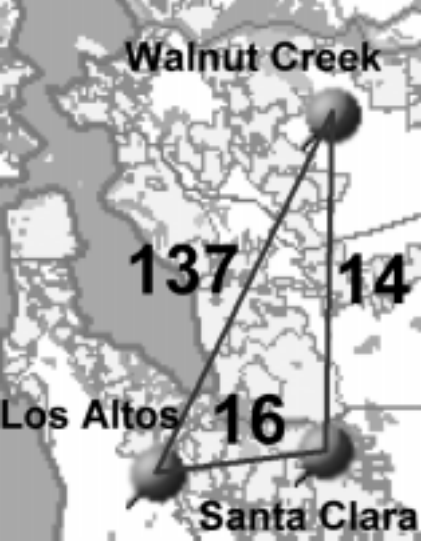
\includegraphics[width=\textwidth]{figures/detour.png} \\
    \textit{Figure from \cite{detour}}
  \end{column}
  \end{columns}
  \note{
    Research in the field has been able to fairly concretely demonstrate the
    problem. Just because your traffic takes a particular route, doesn't mean it
    is going to be the best path for you, in terms of latency or reliability.

    Instead, if you were to route your packets to a ``detour'' and then to the
    final destination, you might actually get path which has better round trip
    time or loss rate. On the right we have an example of a situation found by a
    study, where the default route from Los Altos to Walnut Creek had a round
    trip time of 137 ms, while the combined round trip time of a path via Santa
    Clara was only 30 ms. The reason was that the default route actually
    traveled through Chicago!
  }
\end{frame}

\FigureSlide{figures/detour-packetloss.png}{
  This effect is not limited to isolated examples, either. This same study
  looked at a large group of computers on university networks. They computed
  latency and packet loss rates between each pair of computers. Then, they
  searched for pairs in which the ``triangle inequality'' was violated.

  This graph shows packet loss rates between pairs of computers. The blue is the
  default Internet routed path, and the yellow is the best alternative path that
  uses a single detour. Most of the yellow dots are actually on the zero line.

  You can see here that for a large majority of pairs, there is an alternative
  route that is more reliable. For a small fraction here, the difference in
  reliability is actually huge.
}

\begin{frame}
  \frametitle{Access Link Underutilization}

  \begin{itemize}
  \item Fiber-to-the-home is coming!
  \item However, residential bandwidth is not fully utilized
    \cite{fibertothehome}
    \begin{itemize}
    \item Short-lived TCP sessions?
    \item Small TCP initial window?
    \item Network core can't support bandwidth?
    \end{itemize}
  \item Using alternative routes can improve performance
  \item Aggregating multiple routes can perform even better
  \end{itemize}

  \note{
    Now let's take a brief detour and discuss something else. Recently, we've
    been seeing some exciting trends in residential bandwidth. New access links
    are always being created, and the latest improvement is fiber to the home.
    These can provide up to Gigabit speeds to a home network. However, we've
    had studies right here at CWRU showing that these residential links don't
    use most of that capacity.

    There are several good explanations for this. Short lived TCP sessions may
    never leave the slow-start stage. A small TCP initial window will limit the
    throughput that can be achieved in a reasonable amount of time. But there's
    also the possibility that the network core is becoming the bottleneck for
    some of these connections.

    Two things seem to follow. First, there are good chances that a detour route
    could provide better throughput for a TCP connection, as studies have
    already demonstrated. Second, if we have extra access link capacity, why not
    use these paths in combination with each other, rather than choosing only
    one?
  }
\end{frame}

\begin{frame}
  \frametitle{Contributions}

  \textbf{Problem:} Internet routing inefficiencies can prevent TCP connections
  from achieving their full potential throughput.

  \vspace{0.5cm}

  \textbf{Solution:} A system which can use and aggregate alternative routes for
  TCP connections.

  \vspace{0.5cm}

  \textbf{Contributions:}

  \begin{itemize}
  \item A mechanism for adding alternative routes to Multipath TCP (MPTCP)
    sessions among single-homed hosts.
  \item An evaluation of this mechanism on emulated and real-world networks.
  \end{itemize}
  \note{
    Putting this together, we have a problem: routing inefficiencies can prevent
    TCP connections from achieving their full potential throughput. Access links
    may be capable of much better bandwidth than a user actually gets.

    Our solution is to create a system which can use and aggregate alternative
    paths for TCP connections. Using these paths means that it can route traffic
    along them. Aggregation means combining the potential throughput of both
    paths, to get better throughput than either.

    The contributions this thesis makes are twofold: first, a mechanism that
    allows single-homed devices to add subflows along alternative routes via
    MPTCP. Second, an evaluation of this system on emulated and real world
    networks.
  }
\end{frame}

\section{Background}

\begin{frame}
  \frametitle{Multipath TCP}

  \begin{itemize}
  \item Multi-homed devices are becoming more common
    \begin{itemize}
    \item Smartphones
    \item Datacenters
    \item Laptops
    \end{itemize}
  \item TCP still views a connection as a five-tuple: (TCP, Source IP, Source
    port, Destination IP, Destination Port)
  \item Multi-homed devices are forced to choose a network interface
  \item Multipath TCP is an extension to TCP, allowing hosts to use multiple
    addresses in the same connection
  \end{itemize}
    \note{
      Recently, we've seen a rise in devices that have multiple ways to connect
      to the Internet, network interfaces. For instance, smartphones include
      cellular and WiFi radios, and can be connected to the Internet on both.
      Recent data centers have been taking advantage of multiple interfaces and
      highly redundant network topologies. Laptops can also contain WiFi,
      Ethernet, and even cellular radios.

      Unfortunately, TCP was designed for a simpler time, when computers had a
      single interface and their addresses never changed. This forces
      multi-homed devices to decide which interface they'll use and stick to
      that choice.

      Multipath TCP aims to solve this problem. It is an extension to TCP (not a
      replacement) that allows devices to make use of all of their network
      interfaces and addresses in a single connection.
    }
\end{frame}

\section{Related Work}
\section{Implementation}
\section{Evaluation}
\section{Conclusion}

\appendix % slide numbering includes nothing after here

\section{References}
\begin{frame}[allowframebreaks]
  \frametitle{References}
  \bibliographystyle{ieeetr}
  \bibliography{paper.bib}
\end{frame}

\end{document}